\documentclass[11pt]{article}
\usepackage[utf8]{inputenc}
\usepackage{fourier}
\usepackage{natbib}
\usepackage[top=2.7cm, bottom=2.7cm, left=2.5cm, right=2.5cm]{geometry}
\usepackage{graphicx}
\usepackage{authblk}

\sloppy

\title{\textbf{Machine Learning and Data Mining with the Apache Spark Big Data platform}}
\author{Benjamin Fovet, Maxime Gasque, François Horel, Héloïse Hourquebie, Abderrahman Lahjouji, Anass Seddiki}
\affil{\texttt{\{bfovet, mgasque, fhorel, hhourquebie, alahjouji, aseddiki\} @enseirb-matmeca.fr}}
\date{}

\begin{document}

\maketitle

\textbf{Abstract.} This paper deals with the concepts of \textbf{\textit{machine learning}} and \textbf{\textit{data mining}} social networks, which are increasingly useful for businesses to know the consumers' sentiment towards their brand. This project, intended for use by engineers at Orange France, focuses on the development of a micro-services architecture built around the open source cluster computing framework Apache Spark. Thanks to is distributed model, Spark can process massive amounts of data stored in databases as well as real time data streamed from social networks such as Twitter, Facebook and Orange forum websites. These data are then stored in a cluster database and exposed by an Application Programming Interface (API) server for users to see them in real time.


\section{Context}
% What is Big Data ? (short intro)
Big data is a term used to designate data that is not only too voluminous to fit in a standard database, but is also too diverse and appears at such speed that it cannot be processed using mainstream systems. [Big data now, 2012 edition]

% Orange wants to use Apache Spark
Currently, Orange France is a company already working on big data applications and is interested in using emerging big data technologies. More precisely, among those technologies available today, Apache Spark is the most promising one thanks to its processing performances that makes it well suited to machine learning algorithms.

% What is Apache Spark ? What are the possibilities ? How does it work ?
\subsection{Apache Spark}
Apache Spark is a distributed and highly scalable in-memory system, providing the ability to develop applications using languages like Java, Scala (the language used to write Spark itself), Python and R. It was originally developed at the University of California, Berkeley and donated to the Apache Software Foundation in 2013.
Spark actually consists of four main interoperable components. The figure \ref{spark-stack} below shows the modules built on top of the Spark Core.

\begin{figure}[h!]
    \centering
    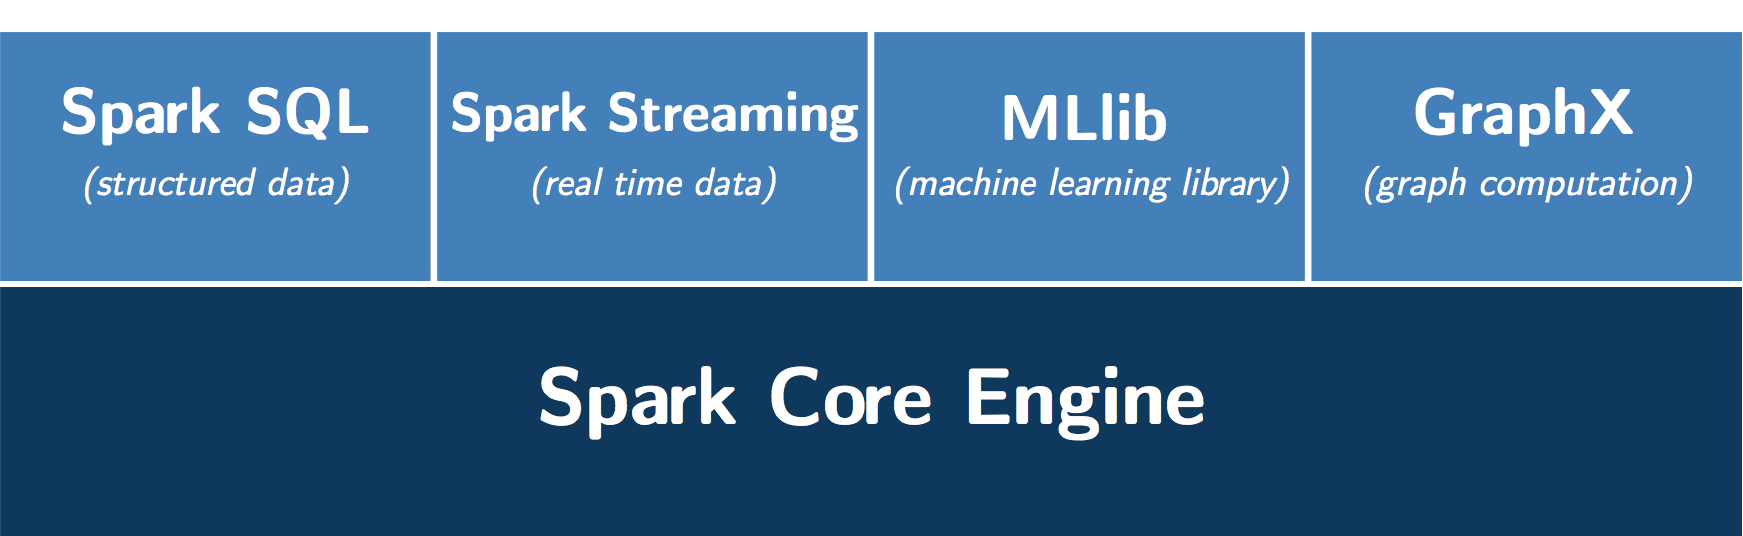
\includegraphics[scale=0.25]{img/spark-stack.eps}
    \caption{The Spark stack}
    \label{spark-stack}
\end{figure}

Spark Core is the foundation of the Spark project and contains functionalities such as task scheduling, memory management, fault recovery and more. On top of that lies four submodules.
Spark SQL is Spark's package for working with structured data which allows SQL queries on many sources of data.
Spark Streaming leverages Spark Core capabilities to enable processing of live streams of data. It is used extensively in this project for fetching data from social networks.
MLlib is a library containing machine learning algorithms that can be applied to compute statistical models from data.
Finally, GraphX is another library for manipulating graphs and performing graph computations.

% Our goal is to demonstrate Spark capabilities, effectiveness and usability through use cases
\subsection{Using Spark in real world scenarios}
The goal of this project is to demonstrate Spark capabilities, effectiveness and usability. At first, requirements were not clearly defined as this project is mainly aimed at exploring what can be done with Spark, but they had to match certain expectations from Orange. These requirements, introduced in the next section, take the shape of use cases as well as Spark integration with other tools.

\section{Use cases}
% Video use case
\subsection{Estimating the crowd in Orange stores}

% Social networks use case
\subsection{Data mining social networks}
\subsubsection{Sentiment analysis}

\subsubsection{Specific computed indicators}

% Every component of our architecture
\subsection{Building a micro-services architecture}

% Presentation and schema first

\subsubsection{Docker}

\subsubsection{Spark cluster}

\subsubsection{Cassandra database cluster}

\subsubsection{API}

\subsubsection{ELK stack}

\section{Organization and Management}

\subsection{Methodology}
\subsection{Tools}
\subsection{Issues}

\section{Conclusion}



\bibliographystyle{plain}
\bibliography{references}

\section{Appendices}
\end{document}